%!TEX program = xelatex
% Note: this template must be compiled with XeLaTeX rather than PDFLaTeX
% due to the custom fonts used. The line above should ensure this happens
% automatically, but if it doesn't, your LaTeX editor should have a simple toggle
% to switch to using XeLaTeX.

\documentclass[
	aspectratio=169, % Uncomment to use an aspect ratio of 16:9 (160 mm by 90 mm)
	%aspectratio=43, % Uncomment to use an aspect ratio of 4:3 (128mm by 96mm)
	t, % Top align all slide content by default
	onlytextwidth, % Typeset content in columns at text width
	10pt, % Default font size, use 10pt for the 16:9 aspect ratio and 8pt for the 4:3 aspect ratio
]{beamer}

\usepackage{../ImperialTheme/beamerthemeImperial} % Use the Imperial theme

\def\imagefolder{../ImperialTheme/Images/}

\title{Sparser-mesh computations} % Presentation title to appear on the title slide and left footers

\subtitle{} % Presentation subtitle to appear on the title slide

\author{Víctor Ballester} % Author name(s) to appear on the title slide

\date{\today} % Presentation date to appear on the title slide and right footers

\begin{document}

\begingroup
\setbeamercolor{background canvas}{bg=ICLBlue} % Slide background color
\setbeamercolor{title page title}{fg=white} % Title text color
\setbeamercolor{title page subtitle}{fg=white} % Subtitle text color
\setbeamercolor{author}{fg=white} % Author(s) text color
\setbeamercolor{date}{fg=white} % Date text color
\setbeamertemplate{title page}[logo]{\imagefolder/ICL_Logo_White.pdf} % Imperial logo color, use 'ICL_Logo_White.pdf' for white and 'ICL_Logo_Blue.pdf' for blue
\frame[plain, s]{\titlepage} % Output the title page with no footer ('plain') and vertically distributed text ('s')
\endgroup

\begin{frame}
	\frametitle{New mesh}
	{
		\centering
	  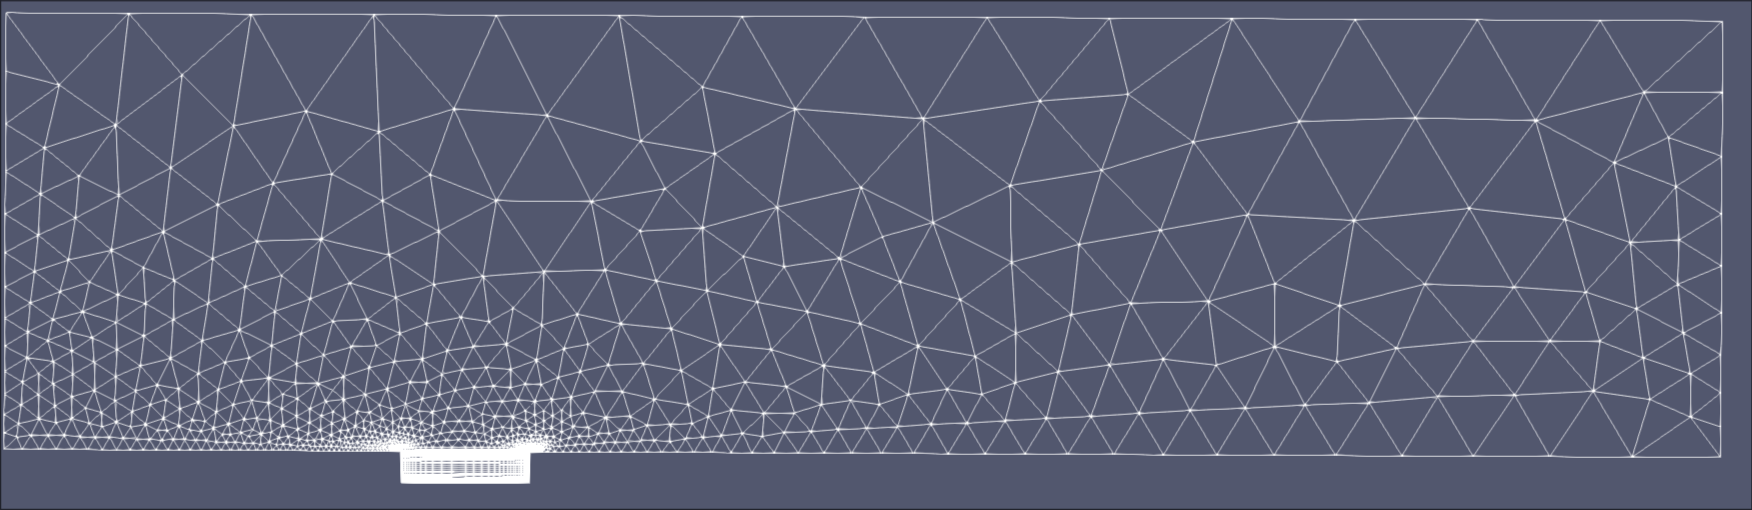
\includegraphics[width=\linewidth]{Images/mesh.png}
  }


  Num elements:  From $\sim24000$ (with the previous mesh) to $\sim3000$!
	One problem is that the downstream region is usually not well resolved.

	Polynomial order for (\textbf{u},p): (7,6) initially and then (9,8) to converge quicker to the Steady State solution.
\end{frame}
\begin{frame}
	\frametitle{New mesh}
	 \centering
	 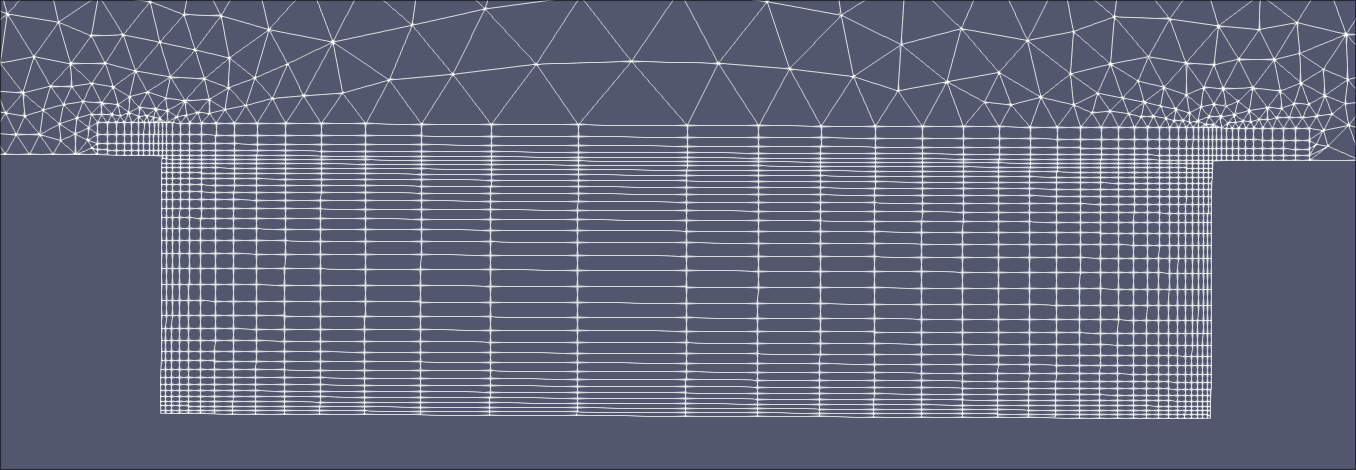
\includegraphics[width=\linewidth]{Images/meshGap.png}
	
\end{frame}
\begin{frame}
	\frametitle{Stability results}
	Everything at $Re_{\delta^*}=1000$.

	Using $D=4\delta^*$, the system with $w=16.25\delta^*$ is stable, but the system with $w=16.5\delta^*$ didn't stabilize (I run it till $t=11574$).

	{
		\centering
		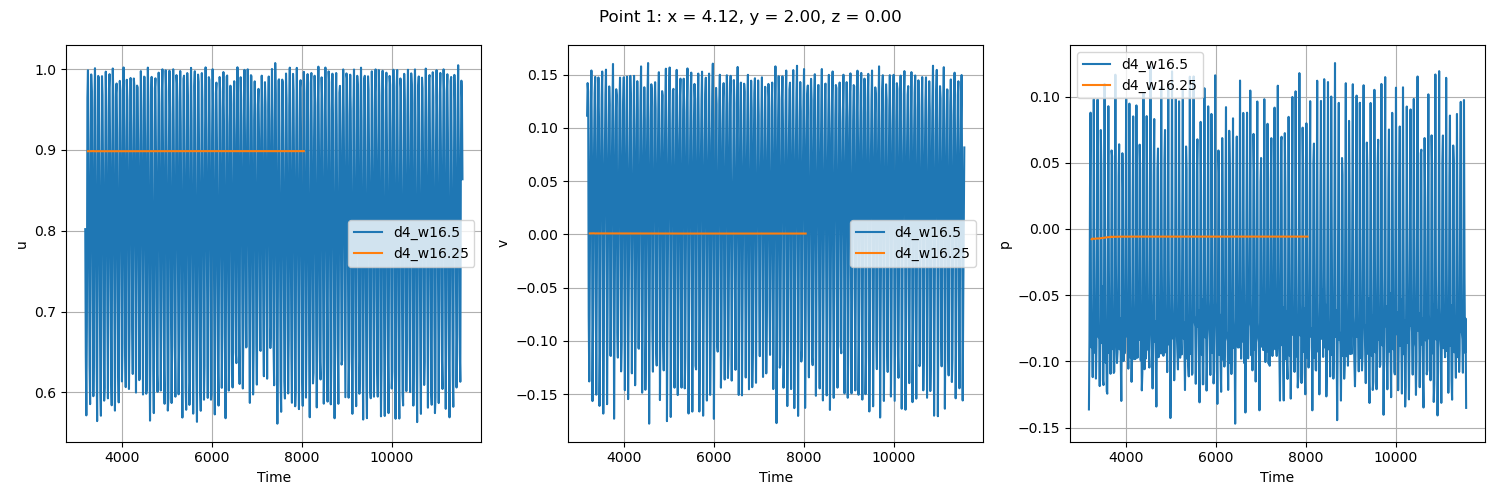
\includegraphics[width=\linewidth]{Images/evolutionU_16.25_16.5.png}
	}

\end{frame}
\begin{frame}
	\frametitle{Stable node $w=16.25\delta^*$}

	\centering
	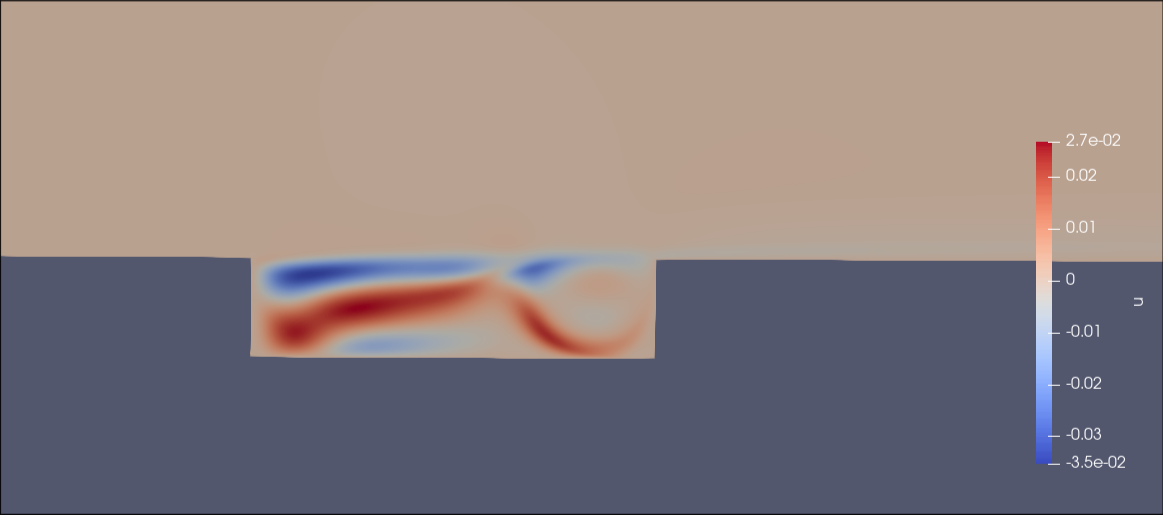
\includegraphics[width=\linewidth]{Images/stablemodeGap16.25.png}
	
\end{frame}
\begin{frame}
	\frametitle{Baseflow $w=16.25\delta^*$}
	
	Vorticity field. 
	{	\centering
	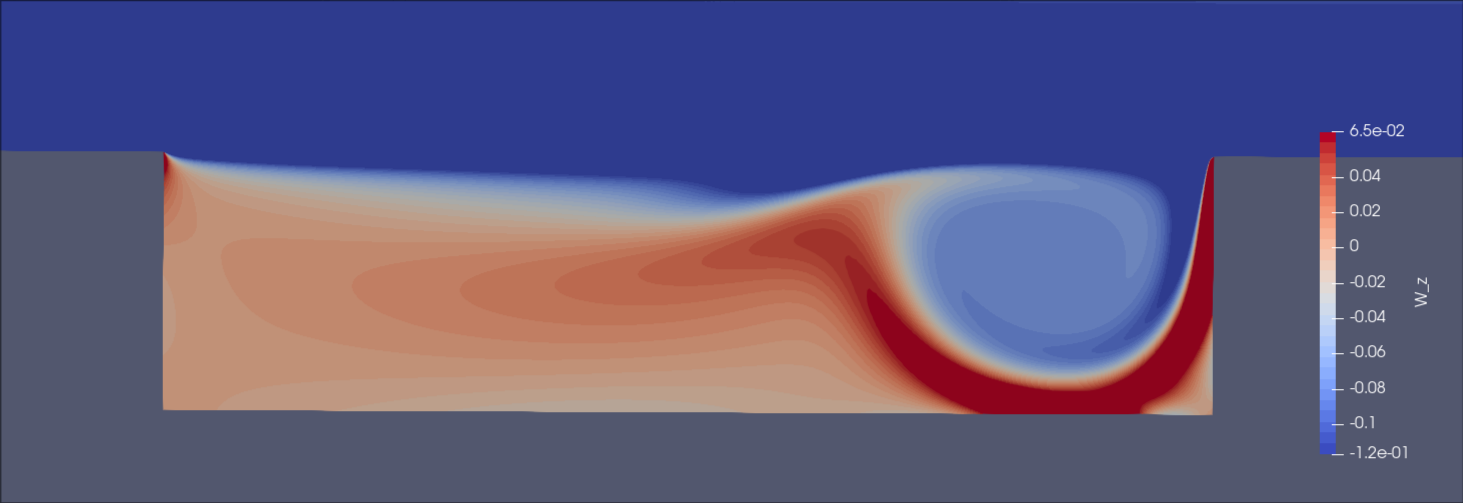
\includegraphics[width=\linewidth]{Images/vorticitybaseflowGap_w16.15.png}}

\end{frame}
\begin{frame}
	\frametitle{Baseflow $w=16.25\delta^*$}
	
	Vorticity field. 
	{	\centering
	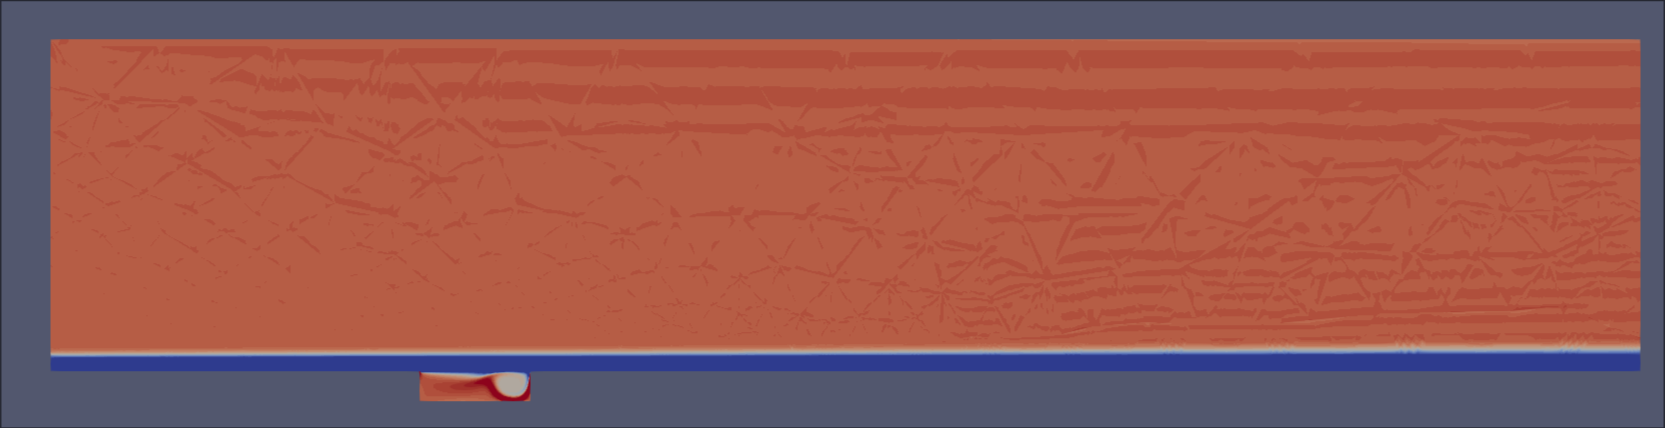
\includegraphics[width=\linewidth]{Images/vorticitybaseflow_w16.15.png}}
	
\end{frame}
\begin{frame}
	\frametitle{Stable node $w=16.25\delta^*$}

	\centering
	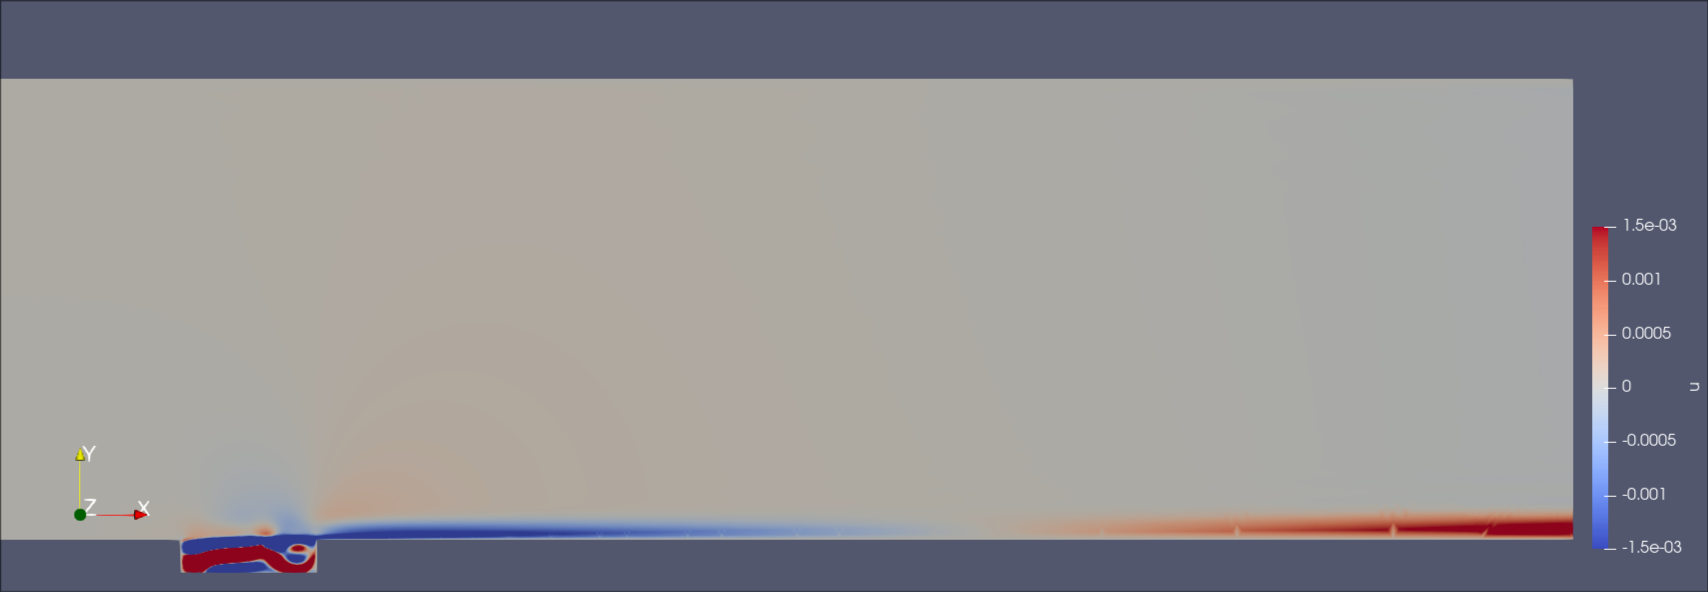
\includegraphics[width=\linewidth]{Images/stablemode16.25.png}

	Does it look ok (the downstream region)?
\end{frame}
\begin{frame}
	\frametitle{Concerns about convergence}

	\begin{itemize}
		\item I stopped the simulation in the steady state solution when the variation in the $u$ component is less than $10^{-7}$. In the linear NavierStokes I stop the computation of the eigenvectors when their residual is of the order of $10^{-5}$.
		\item My concern is that the dependence in the domain aspect ratios is much higher than that. And probably the resolution of the smallest element as well (e.g. order of the polynomials). I want to check this. Any suggestions?
	\end{itemize}
\end{frame}


\end{document}
